\section{\sys Design}
\label{sec:design}

\subsection{Overall Procedure}

Figure~\ref{fig:quiet-overview} follows the same four steps in deployment and
measurement.  First, \sys profiles a concrete workload and freezes its
deadline independently of the evaluated treatments.  Second, it evaluates
candidate stage placements, quotas, transports, and protection scopes, then
serializes exactly one feasible plan.  Third, the runtime follows the
activation lifecycle to acquire and release protection.  Finally, an evidence
pipeline replays every request and promotes a number only after its application,
runtime, comparator, and thermal gates pass.

This separation is deliberate.  Calibration cannot observe the treatment
comparison, and the executor cannot rewrite the selected plan after creating a
CUDA context.  The evidence pipeline cannot repair a failed request or
reinterpret an exploratory campaign as formal.  Each transition carries the
hash of the artifact that authorized it.

\subsection{Full-Coherent Registered System-Memory Activation Edge}
\label{sec:edge}

The harness creates a page-aligned shared \texttt{mmap}.  After selecting its
assigned MIG device, each process registers the complete range with
\texttt{cudaHostRegisterMapped} and obtains a local device address through
\texttt{cudaHostGetDevicePointer}.  The producer binds that address to its
TensorRT output; the consumer binds its own address for the same physical
range to its TensorRT input.  Both call
\texttt{IExecutionContext::setTensorAddress} and execute with
\texttt{enqueueV3}.  The hot path therefore materializes the activation once
in coherent system memory and performs no explicit D2H/H2D bounce.

Publication has two parts.  TensorRT completion establishes that the producer
has finished writing the payload; a control message transfers the request
sequence and readiness state to the consumer.  The consumer cannot launch
before receiving that message.  Alternative pinned-bounce, pageable-bounce,
managed-memory, and host-materialization paths remain explicit controls.
\sys never assumes that registration wins: it records producer visibility,
notification, consumer read, and complete wall latency for each candidate.

Payload identity is request scoped.  A capture run stores producer activations
in the \texttt{JDGACT1} format with request ID, shape, size, and checksum.  An
independent causal arm maps those pre-captured bytes before release, whereas
the dependent arm consumes the live publication.  Model, input, activation
bytes, placement, quota, release, background load, request ID, and output
oracle remain fixed; only precedence changes.  This removes CPU
initialization and timed-path copies as causal confounders.

The separate multi-slot implementation uses three payload slots with
\texttt{FREE}$\rightarrow$\texttt{PRODUCING}$\rightarrow$\texttt{READY}
$\rightarrow$\texttt{CONSUMING}$\rightarrow$\texttt{FREE} ownership,
monotonic sequence numbers, backpressure counters, deadlines, peer-liveness
checks, and stale-slot reclamation.  We use it to validate the data-plane
state machine and failures, but retain the lower-inflight production path for
the formal application campaign.

\subsection{Communication-Aware Placement and Admission}
\label{sec:planner}

A candidate plan is
\begin{equation}
  P=(U_P,U_C,q_P,q_B,T,\Gamma),
\end{equation}
where $U_P$ and $U_C$ are the producer and consumer MIG UUIDs, $q_P$ and $q_B$
are producer and best-effort quotas, $T$ is the edge transport, and $\Gamma$
is the protection scope.  The profile contains stage and edge diagnostics, but
the promotable response bound is the Type-7 p99 of the \emph{joint}
arrival-to-completion samples:
\begin{equation}
  R(P)=Q_{0.99}\!\left(\{L_i(P)\}\right).
  \label{eq:joint-tail}
\end{equation}
Legacy sums of component p99s may guide characterization but cannot authorize
a formal plan.

Let $G(P)$ be the measured p99 time needed to close and drain best-effort
submission, and let $H$ be pre-release lookahead.  The uncovered guard is
\begin{equation}
  U(P)=\max(0,G(P)-H).
\end{equation}
The plan is feasible only if
\begin{equation}
  S(P)=D-R(P)-U(P)\ge 0,
  \label{eq:slack}
\end{equation}
the held-out execution also satisfies its p99 gate, and all artifact and
application bindings match.

The current deadline is frozen from two independent 1,100-request calibration
blocks: the pooled p99 is $2{,}050.439~\mu$s and the predeclared 1.10 factor
gives $D=2{,}255.483~\mu$s.  The selected forward placement runs the
ResNet-50 backbone on 1g and its head on 2g.  Its held-out joint p99 is
$1{,}833.098~\mu$s; $G=2{,}000.588~\mu$s and $H=2{,}300~\mu$s make
$U=0$, leaving $422.385~\mu$s of reserved slack.  The serialized plan binds
these values to the exact deadline lock, engines, UUIDs, quotas, payload size,
transport, and producer-only scope.

Planning precedes process creation.  A CLI override that changes a UUID,
transport, quota, protection scope, deadline, or workload hash fails before a
GPU process is started.  This matters because accepting a mismatched plan and
merely annotating the trace would turn admission into an after-the-fact label.

\subsection{Stage-Aware Quiescence}
\label{sec:quiescence}

\begin{figure}[t]
  \centering
  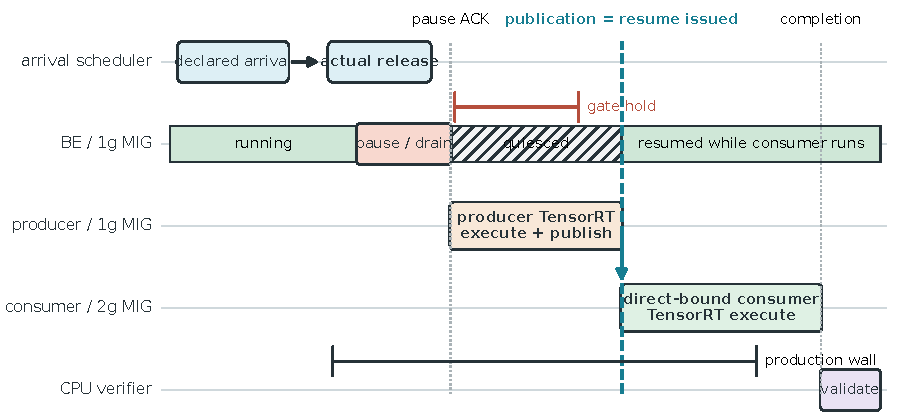
\includegraphics[width=\columnwidth]{figures/p9-stage-timeline.pdf}
  \caption{\sys's request lifecycle.  The operational release precedes gate
  acquisition, so queue and drain delay remain inside the production wall.
  Producer publication is the protection boundary: resume is issued before
  checksum and output validation, and best-effort work overlaps the consumer.}
  \Description{A five-lane timeline shows request release, best-effort drain
  and pause, producer execution and publication, immediate best-effort resume,
  consumer execution, completion, and post-completion validation.}
  \label{fig:stage-timeline}
\end{figure}

Figure~\ref{fig:stage-timeline} shows the runtime protocol.  Before producer
launch, \sys closes future best-effort submission and waits for cooperative
pause acknowledgement.  This is a drain boundary, not a claim of
mid-kernel preemption.  Once acknowledged, the producer executes without new
best-effort work entering its 1g instance.

Producer completion publishes the activation and releases the dependent
consumer.  In the same control transition, \sys issues resume to the
best-effort tenant and records both issue and observation timestamps.  The
consumer then reads the direct-bound payload and executes on 2g while
best-effort work again occupies 1g.  Full-request gating would retain
protection through this interval and forfeit safe work; no gating would expose
the producer tail.  Publication-scoped gating protects exactly the interval
whose interference can delay every downstream stage.

Each event trace records declared arrival, actual release, queue delay,
producer start, publication, consumer start, completion, pause begin and
completion, resume issue and observation, and gate-hold duration.  The
operational \texttt{JDGARR1} scheduler consumes predeclared offsets.  A late
release contributes queue delay rather than shifting the schedule, and neither
an acknowledgement nor post-completion validation determines the next
arrival.

\subsection{Correctness and Evidence Promotion}
\label{sec:evidence}

\sys separates production completion from proof collection without weakening
correctness.  After publication, the producer checks the complete activation
against its request record.  After consumer completion, the harness captures
the complete output and evaluates the application oracle.  A run fails on a
request-sequence mismatch, activation mismatch, output mismatch, stale hash,
missing sensor, or fewer requests than declared.

Promotion has three levels.  A \emph{mechanism control} validates behavior
such as ring recovery or transport direction.  An \emph{exploratory result}
adds repeated measurements but lacks at least one formal condition, such as
thermal normalization or sufficient confidence.  A \emph{formal result} binds
the current binary and engines, operational releases, application inputs and
outputs, balanced treatment order, independent sessions, thermal sensors, and
an exact deadline-miss confidence bound.  Results never cross levels during
aggregation.
